\documentclass[usenames,dvipsnames]{beamer}


\usepackage{amsmath,amssymb,graphics,graphicx}
%\usepackage{hyperref}
%\usepackage{epigraph}
%\usepackage{mdwlist}
\usepackage{style/preamble}
%\usepackage{hyperref}
\usepackage{color}
\definecolor{mydarkblue}{rgb}{0,0.08,0.45}
\hypersetup{ %
    colorlinks=true,
    linkcolor=mydarkblue,
    citecolor=mydarkblue,
    filecolor=mydarkblue,
    urlcolor=mydarkblue}
\pdfmapfile{+sansmathaccent.map}

\setbeamertemplate{blocks}[rounded][shadow=true]
\beamertemplatenavigationsymbolsempty

%%%%%%%%%%%%%%%%%%%%%%%%%%
% Beamer template options
%%%%%%%%%%%%%%%%%%%%%%%%%%

\setbeamertemplate{items}[circle]

%%%%%%%%%%%%%%%%%%%%%%%%%%
% Unused but may be useful in future
%%%%%%%%%%%%%%%%%%%%%%%%%%

\newenvironment{custommargins}[2]%
  {\addtolength{\leftskip}{#1}\addtolength{\rightskip}{#2}}{\par}
  
%%%%%%%%%%%%%%%%%%%%%%%%%%
% Pseudo constants
%%%%%%%%%%%%%%%%%%%%%%%%%%

\newcommand{\standardspace}{
  0.03\textwidth
}

\newcommand{\standardtwocolumnwidth}{
  0.45\textwidth
}

\definecolor{beamerblue}{rgb}{0.2,0.2,0.7}

%%%%%%%%%%%%%%%%%%%%%%%%%%
% Layout
%%%%%%%%%%%%%%%%%%%%%%%%%%

\newcommand{\spacer}[1]{
  \begin{minipage}{#1}
    \hspace{#1}
  \end{minipage}
}

\newcommand{\titlebodyskip}{
  \begin{minipage}[t][\baselineskip][t]{\textwidth}
  \end{minipage}
}

\newcommand{\headerbar}[1]{
  \begin{minipage}[t][2.0\baselineskip][b]{1\textwidth}
    #1
  \end{minipage}
}

\newcommand{\bodyheaderskip}{
	\begin{minipage}[t][\baselineskip][t]{\textwidth}
	\end{minipage}
}

\newcommand{\slidebody}[1]{
  \begin{minipage}[t][0.45\paperheight][t]{\textwidth}
    #1
  \end{minipage}
}

%%%%%%%%%%%%%%%%%%%%%%%%%%
% Slide elements
%%%%%%%%%%%%%%%%%%%%%%%%%%

\newcommand{\frametitleJL}[1]{
  \begin{minipage}[t][2.0\baselineskip][b]{\textwidth}
  {
    \color{beamerblue}
    \large
    #1
  }
  \end{minipage}
}

\newcommand{\columnheader}[2]{
  \begin{minipage}[b]{#1}
  {
  \small
  \begin{center}
    \textbf{#2}
    \end{center}
    \vspace{-2.3\baselineskip}
    \begin{center}
      {\color{beamerblue} \rule{\linewidth}{1pt}}
    \end{center}
  }
  \end{minipage}
}

\newcommand{\columnbody}[2]{
  \begin{minipage}[t][0.45\paperheight][t]{#1}
    \vspace{0.000001\baselineskip}
    {\footnotesize #2}
  \end{minipage}
}

\newcommand{\takeaway}[1]{
  \spacer{0.13\textwidth}
  \begin{minipage}[t][2\baselineskip][c]{0.70\textwidth}
  {
    \small
    \begin{center}
    {
      \color{beamerblue}
      \textbf{#1}
    }	
    \end{center}
  }
  \end{minipage}
  \spacer{0.13\textwidth}
}



\begin{document}

%%%%%%%%%%%%%%%%%%%%%%%%%%%%%%%%%
% Commands to insert agenda slides
%%%%%%%%%%%%%%%%%%%%%%%%%%%%%%%%%

\AtBeginSection{
	\begin{frame}
		\frametitleJL{Agenda}
		\tableofcontents[currentsection]
	\end{frame}
}

\AtBeginSubsection{
	\begin{frame}
		\frametitleJL{Agenda}
		\tableofcontents[currentsubsection]
	\end{frame}
}

%%%%%%%%%%%%%%%%%%%%%%%%%%%%%%%%%
% Title page
%%%%%%%%%%%%%%%%%%%%%%%%%%%%%%%%%

\title{\textbf{Deterministic Sampling Methods}}
\author{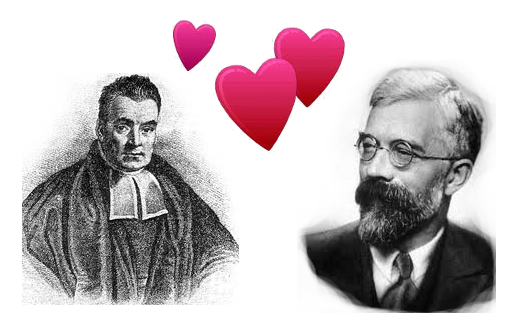
\includegraphics[width=0.6\textwidth]{figures/fisherbayes/lovers2}
\\David Duvenaud} 
 
\institute{Cambridge University
\\Computational and Biological Learning Lab}

\begin{frame}
	\titlepage
\end{frame}

%%%%%%%%%%%%%%%%%%%%%%%%%%%%%%%%%
% Table of contents
%%%%%%%%%%%%%%%%%%%%%%%%%%%%%%%%%

%%%%%%%%%%%%%%%%%%%%%%%%%%%%%%%%%
% Slides
%%%%%%%%%%%%%%%%%%%%%%%%%%%%%%%%%



\begin{frame}[plain, t]
	\frametitleJL{Outline}
	%
	\bodyheaderskip
	%
	\slidebody
	{
		\begin{itemize}
			\item Kernel Herding
			\item Bayesian Quadrature			
			\item Unifying Results
			\item Demos
		\end{itemize}
	}
	%
%	\takeaway%
%{
%	Takeaway
%}
\end{frame}


%\begin{frame}[plain, t]
%	\frametitleJL{The Quadrature problem}
	%
%	\bodyheaderskip
	%
%	\slidebody
%	{

%		\item Approximate inference is a huge part of the machine learning research project.
%		\end{itemize}
%	}
	%
%	\takeaway%
%{
%	Takeaway
%}
%\end{frame}


\begin{frame}[plain, t]
	\frametitleJL{The Quadrature Problem}
	%
	\titlebodyskip
	%
	\headerbar
	{

	}
	%
	\bodyheaderskip
	%
	\slidebody
	{
		\columnbody{\standardtwocolumnwidth}
		{		
			\begin{itemize}
%		\begin{itemize}
		\item We want to estimate an integral $$Z = \int f(x) p(x) dx$$		
		\item Most computational problems in Bayesian inference correspond to integrals:
			\begin{itemize}
			\item Expectations
			\item Marginal distributions
			\item Integrating out nuisance parameters
			\item Normalization constants
		\end{itemize}			
%				\end{itemize}			
	
		%	\only<2>{\item Several ways to learn about or summarize $f(x)$ in order to approximate $Z$.		
		%	\item Expectation Propagation, Laplace approximation, Variational Bayes are some non-sampling approaches.}
			\end{itemize}   		
		}
		%
		\spacer{\standardspace}
		%
		\columnbody{\standardtwocolumnwidth}
		{
			\vskip10pt
       		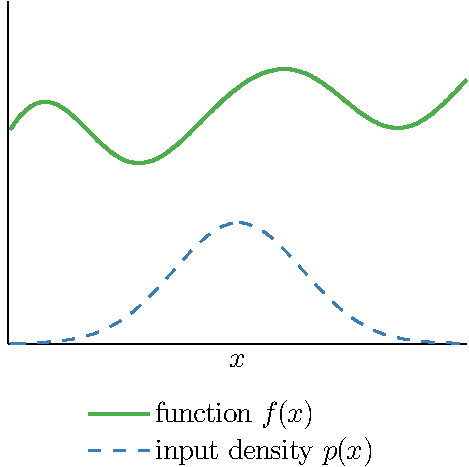
\includegraphics[width=4.5cm]{figures/samples/no_sample}	
		}
	}
	%
%	\takeaway%
%{
%	Takeaway
%}
\end{frame}



\begin{frame}[plain, t]
	\frametitleJL{Sampling Methods}
	%
	\titlebodyskip
	%
	\headerbar
	{
%		\columnheader{\standardtwocolumnwidth}
%		{
%			Simple Monte Carlo
%		}
		%
%		\spacer{\standardspace}
		%
%		\columnheader{\standardtwocolumnwidth}
%		{
%			Simple Monte Carlo
%		}
	}
	%
	\bodyheaderskip
	%
	\slidebody
	{
		\columnbody{\standardtwocolumnwidth}
		{		
			\begin{itemize}
			\item Monte Carlo methods:  Sample from $p(x)$, take empirical mean: $$\hat{Z} = \frac{1}{N} \sum_{i=1}^N f(x_i)$$
			\only<2-5>{	\item Possibly sub-optimal for two reasons:}
				\only<3-5>{\begin{itemize}
					\item Random bunching up
					\only<4-5>{\item Often, nearby function values will be similar}
				\end{itemize}}							
			\only<5>{\item Quasi-Monte Carlo methods spread out samples to achieve faster convergence.}	
			\end{itemize}   		
		}
		%
		\spacer{\standardspace}
		%
		\columnbody{\standardtwocolumnwidth}
		{
			\vskip10pt
       		\only<1>{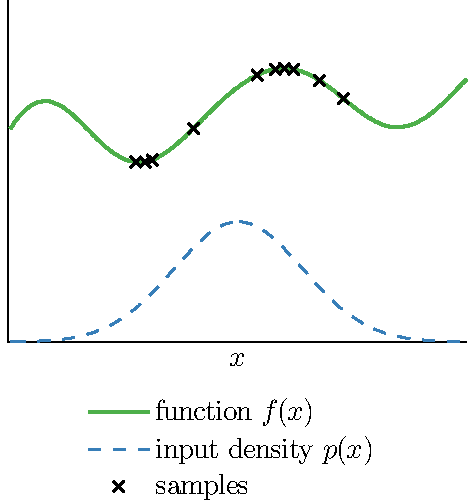
\includegraphics[width=4.5cm]{figures/samples/mc_sample}}
     		\only<2-4>{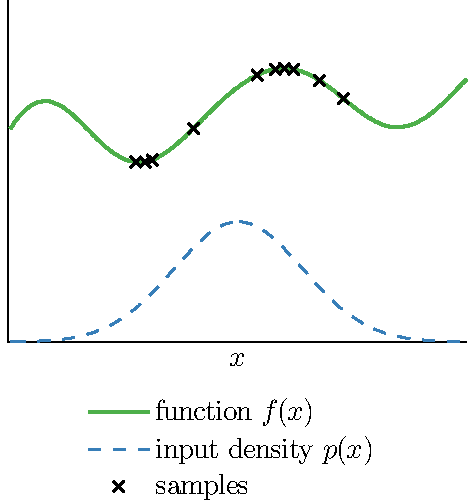
\includegraphics[width=4.5cm]{figures/samples/mc_sample}}
       		\only<5>{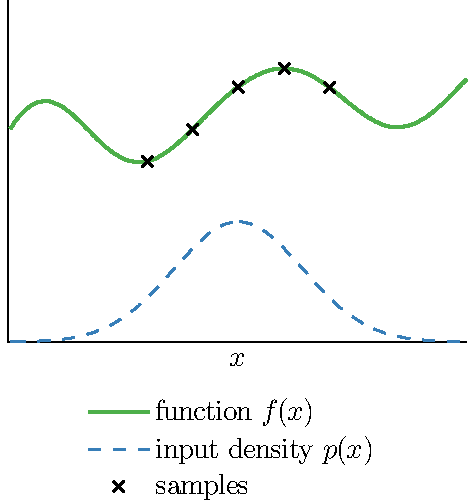
\includegraphics[width=4.5cm]{figures/samples/herd_sample}}		
		}
	}
	%
%	\takeaway%
%{
%	Takeaway
%}
\end{frame}



\begin{frame}[plain, t]
	\frametitleJL{Kernel Herding [Welling et. al., 2009, Chen et. al., 2010]}
	%
	\bodyheaderskip
	%
	\slidebody
	{
		\begin{itemize}
			\item A sequential procedure for choosing sample locations, depending on previous locations.
			\pause			
			\item Keeps estimate rule $\hat{Z} = \frac{1}{N} \sum_{i=1}^N f(x_i)$
			\pause			
			\item Almost $\mathcal{O}(1/N)$ convergence instead of $\mathcal{O}(1/\sqrt{N})$ typical of random sampling, by spreading out samples.
		\end{itemize}
		\centering			
		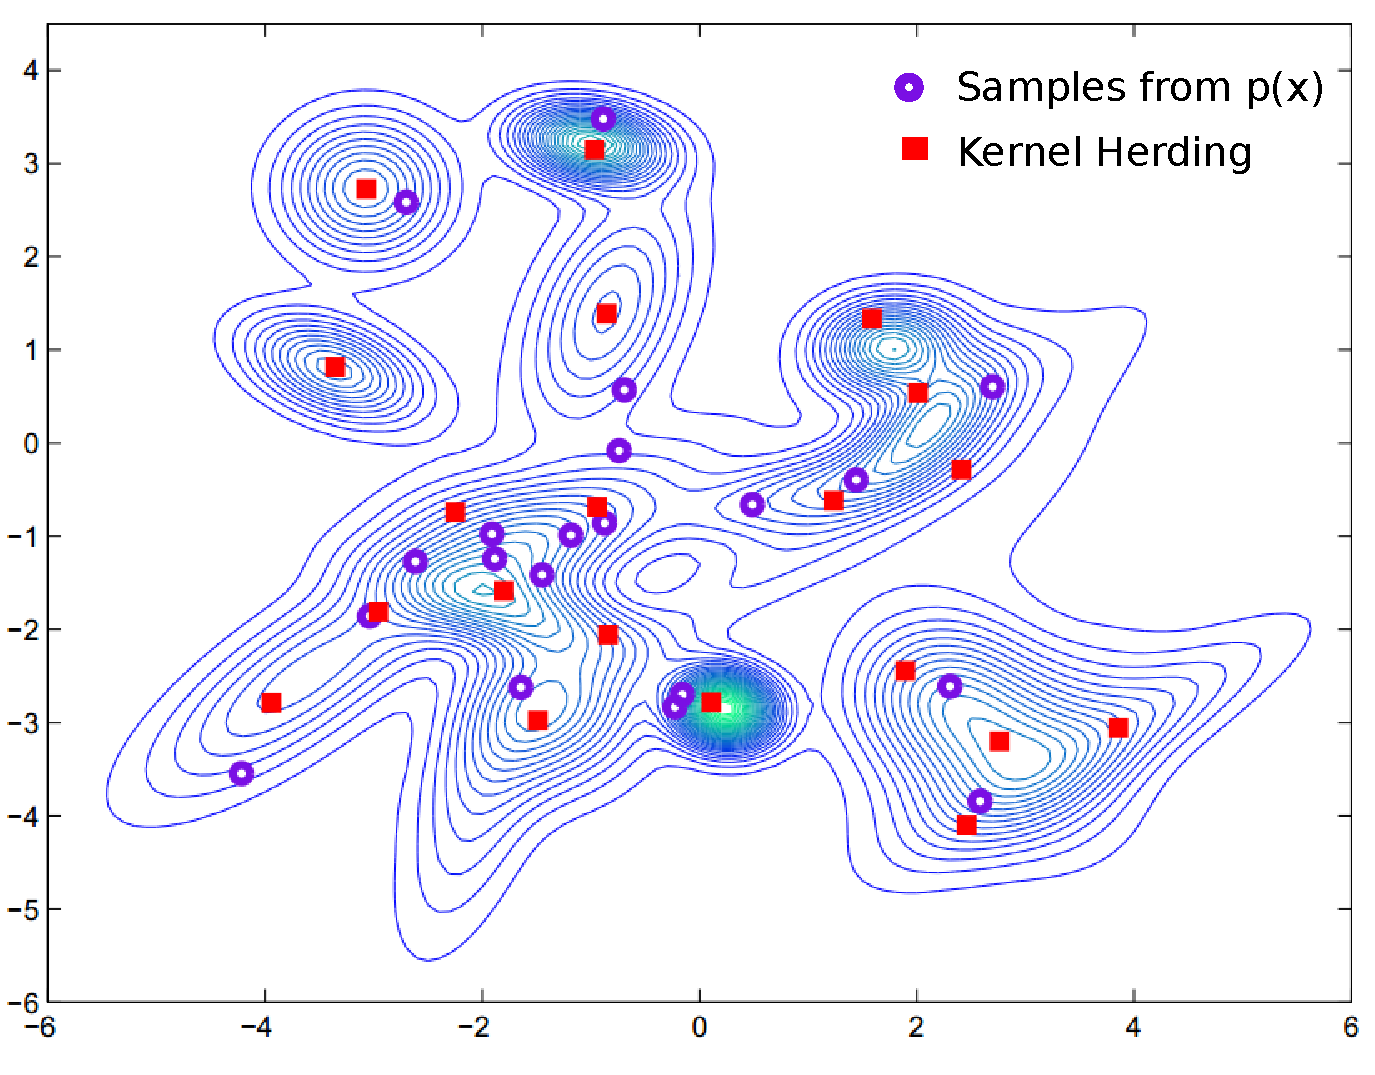
\includegraphics[width=6cm]{figures/kh_samples_legend} \\
	}
	%
%	\takeaway%
%{
%	Takeaway
%}
\end{frame}



\begin{frame}[plain, t]
	\frametitleJL{Kernel Herding Objective}
	%
	\titlebodyskip
	%
%	\bodyheaderskip
	%
	%Assumes function is in a RKHS defined by $k(\cdot , \cdot)$	
	\slidebody
	{
		KH was found to minimize Maximum Mean Discrepancy:
		\begin{align*}
			\mmd_{\mathcal{H}}\left(p,q\right) = \sup_{\substack{f\in\He\\\Hnorm{f}=1}}\left\vert\int f(x) p(x) dx - \int f(x) q(x) dx \right\vert
		\end{align*}
		\pause
		In KH, $p(x)$ is true distribution, and $q(x)$ is a set of point masses at sample locations $\{\vx_1,\ldots,\vx_{N}\}$:
		\begin{align*}
			\epsilon_{KH}&\left(\{\vx_1,\ldots,\vx_{N}\}\right) = 
			\mmd_{\He}\left(p, \underbrace{\frac{1}{N}\sum_{n=1}^{N}\delta_{x_n}}_{q(x)}\right)
		\end{align*}
	}
	%
%	\takeaway%
%{
%	Takeaway
%}
\end{frame}




\begin{frame}[plain, t]
	\frametitleJL{Kernel Herding}
	%
	\titlebodyskip
	%
%	\bodyheaderskip
	%
	%Assumes function is in a RKHS defined by $k(\cdot , \cdot)$	
	\slidebody
	{
	\begin{itemize}
\item 		Assuming function is in a Reproducing Kernel Hilbert Space defined by $k(\cdot , \cdot)$, MMD has closed form.
		
%		\begin{align*}
%			\mmd_{k(\cdot , \cdot)}\left(p, \frac{1}{N}\sum_{n=1}^{N}\delta_{x_n}\right)
%		 	%& = \expectargs{\vx, \vx' \sim p}{k(\vx, \vx')} \\
%		 	& = \int \!\!\! \int k(\vx, \vx') p(x) p(x') dx dx' \\
%			& \quad -2 \frac{1}{N}\sum_{n=1}^{N}\int k(x,x_n) p(x) dx \\
%			& \quad + \frac{1}{N^2}\sum_{n,m=1}^{N} k(x_n,x_m)
%		\end{align*}

\pause

\item When sequentially minimizing MMD, new point is added at:
\begin{align*}
%\nonumber \vx_{n+1} & = \argmin_{\vx \in \mathcal{X}} \mmd \left( p, \frac{1}{N}\sum_{n=1}^{N+1}\delta_{x_n} 5\right) \\
%& = \argmax_{\vx \in \mathcal{X}} 2 \expectargs{\vx' \sim p}{k(\vx, \vx')} \nonumber \\
x_{N+1} = \argmax_{\vx \in \mathcal{X}} \bigg[ 2 \! \int \! k(\vx, \vx') p(x') dx' \nonumber - \frac{1}{N+1}\sum_{m=1}^{N} k(\vx,\vx_m) \bigg]\\
\end{align*}
\end{itemize}
	}
	%
%	\takeaway%
%{
%	Takeaway
%}
\end{frame}


\begin{frame}[plain, t]
	\frametitleJL{Kernel Herding in Action}
	%
	\titlebodyskip
	%
%	\headerbar
%	{
	%	\columnheader{\standardtwocolumnwidth}
		%{
	%		A sequential method
%		}
		%
	%	\spacer{\standardspace}
		%
%		\columnheader{\standardtwocolumnwidth}
%		{
%			Kernel Herding [cite]
%		}
%	}
	%
	\bodyheaderskip
	%
	\slidebody
	{
		\columnbody{\standardtwocolumnwidth}
		{		
%Adds one point at a time, greedily minimizing $$\mmd_{k}\left(p, \frac{1}{N}\sum_{n=1}^{N}\delta_{x_n}\right)$$
%
%Other terms remaining constant, new point added at:

New point is added at:
\begin{align*}
%\nonumber \vx_{n+1} & = \argmin_{\vx \in \mathcal{X}} \mmd \left( p, \frac{1}{N}\sum_{n=1}^{N+1}\delta_{x_n} 5\right) \\
%& = \argmax_{\vx \in \mathcal{X}} 2 \expectargs{\vx' \sim p}{k(\vx, \vx')} \nonumber \\
& x_{N+1} = \\
& \argmax_{\vx \in \mathcal{X}} \bigg[ 2 \! \int \! k(\vx, \vx') p(x') dx' \nonumber \\
\nonumber & \quad \quad \qquad - \frac{1}{N+1}\sum_{m=1}^{N} k(\vx,\vx_m) \bigg]\\
\end{align*}		
		}
		%
		\spacer{\standardspace}
		%
		\columnbody{\standardtwocolumnwidth}
		{
       		\only<1>{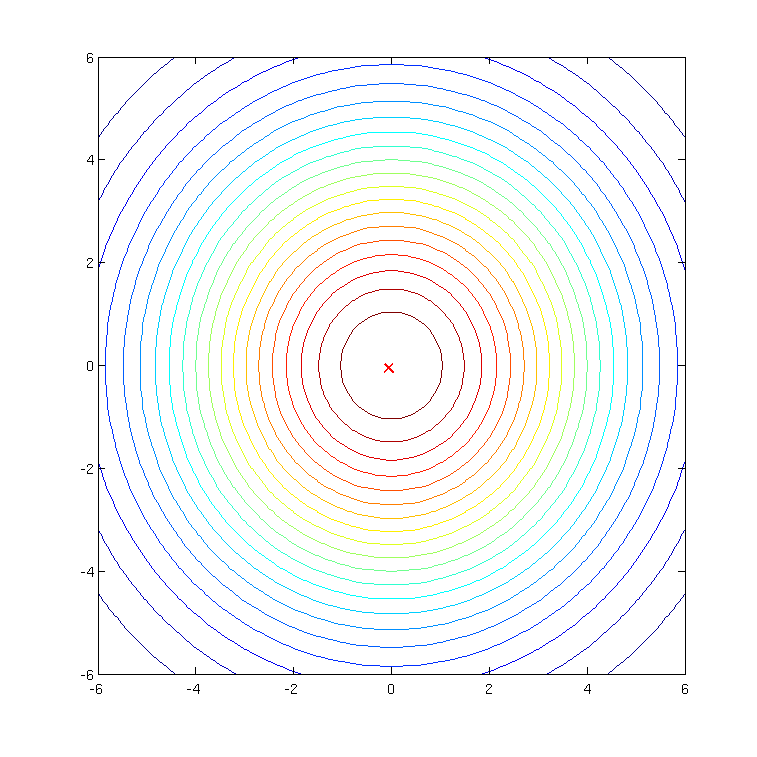
\includegraphics[width=6cm]{figures/herd_movie/v2herd1}}
       		\only<2>{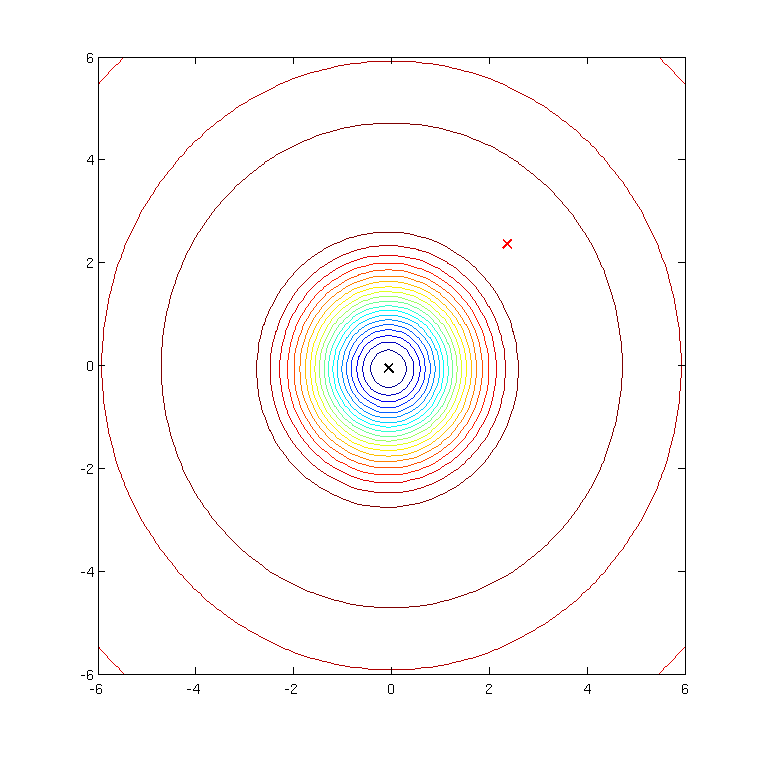
\includegraphics[width=6cm]{figures/herd_movie/v2herd2}}
       		\only<3>{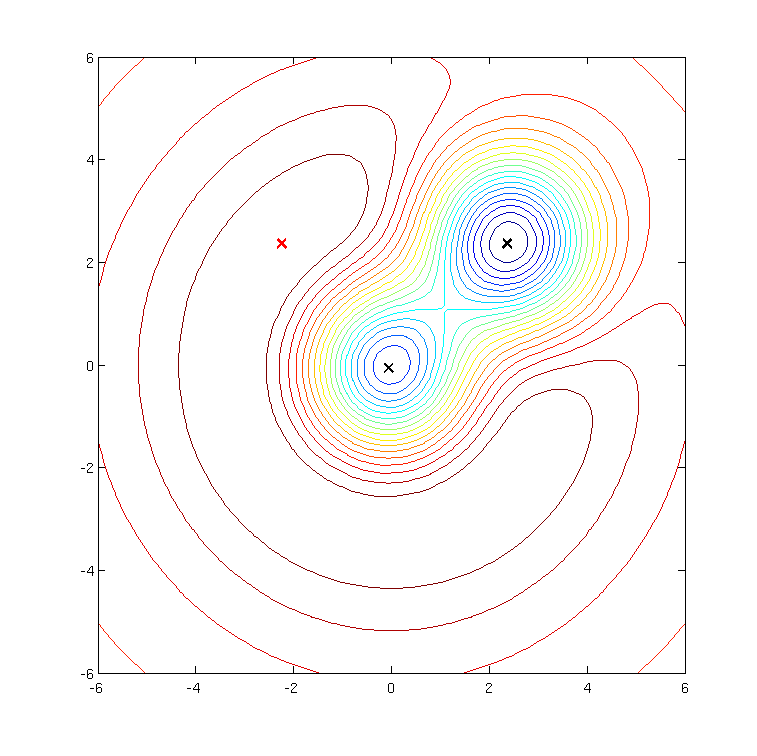
\includegraphics[width=6cm]{figures/herd_movie/v2herd3}}
       		\only<4>{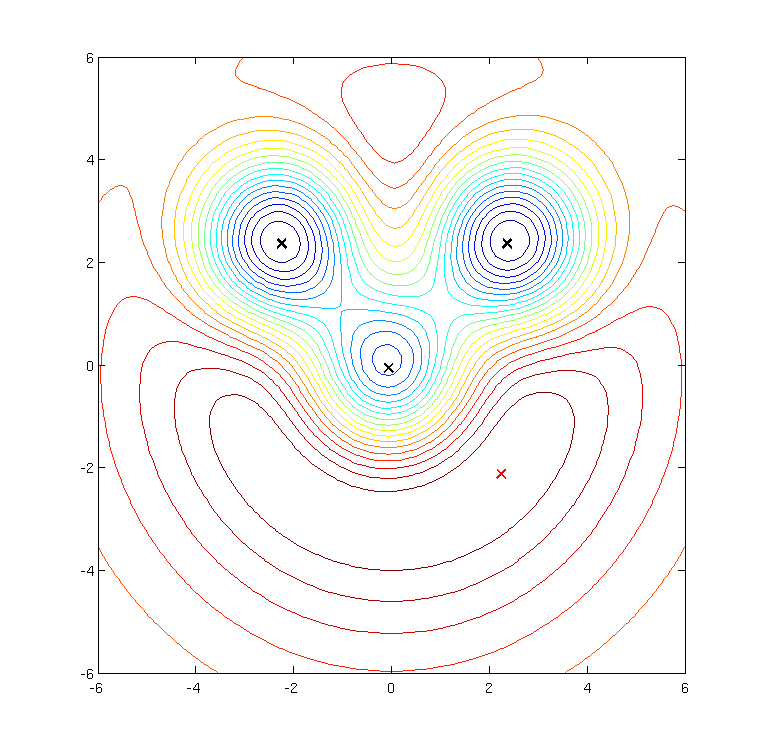
\includegraphics[width=6cm]{figures/herd_movie/v2herd4}}
       		\only<5>{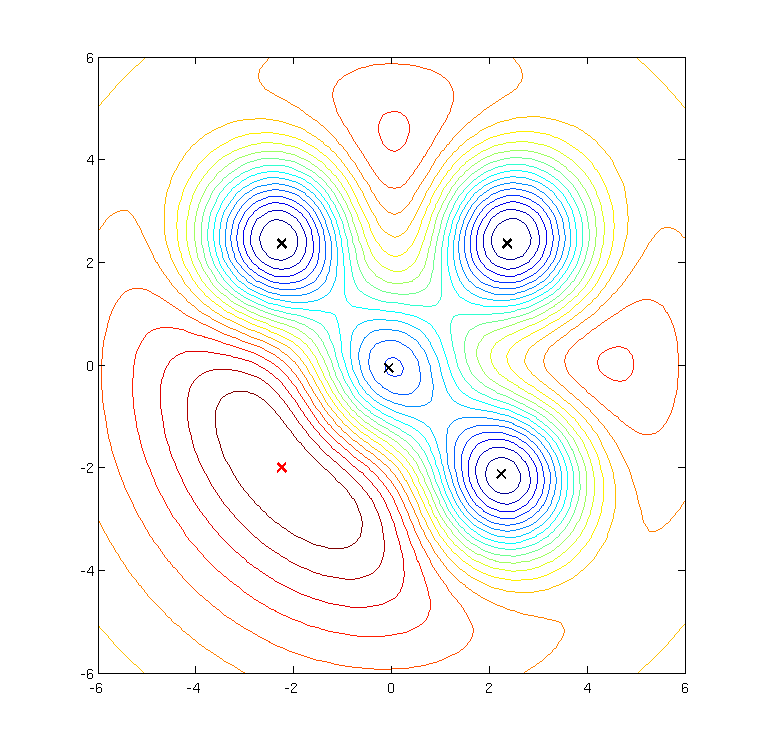
\includegraphics[width=6cm]{figures/herd_movie/v2herd5}}
       		\only<6>{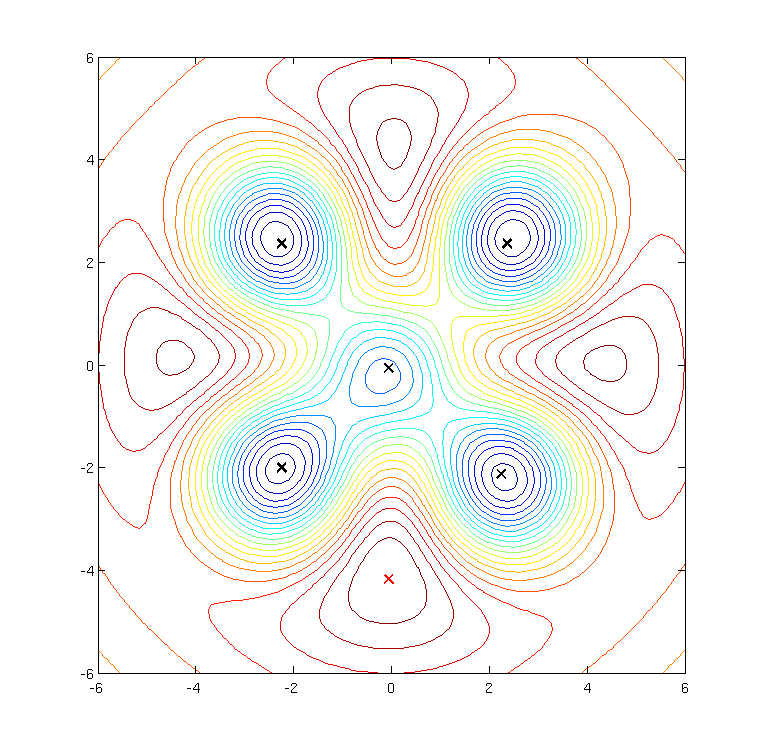
\includegraphics[width=6cm]{figures/herd_movie/v2herd6}}
       		\only<7>{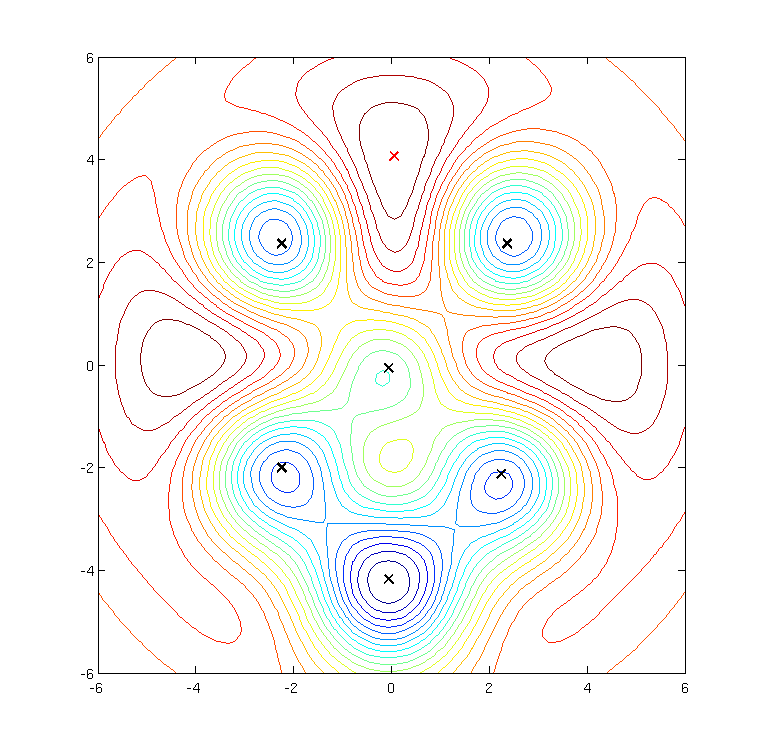
\includegraphics[width=6cm]{figures/herd_movie/v2herd7}}
       		\only<8>{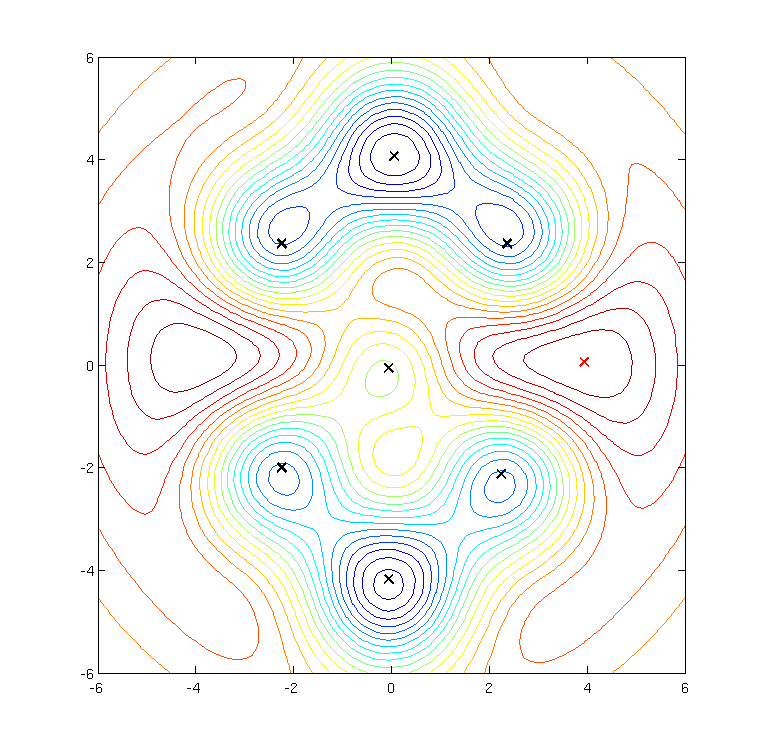
\includegraphics[width=6cm]{figures/herd_movie/v2herd8}}
       		\only<9>{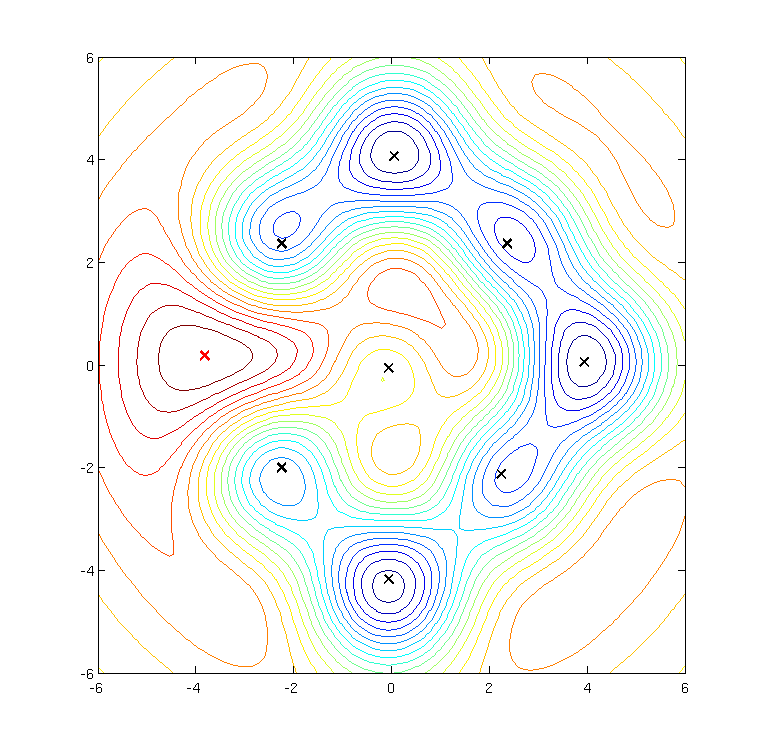
\includegraphics[width=6cm]{figures/herd_movie/v2herd9}}
       		\only<10>{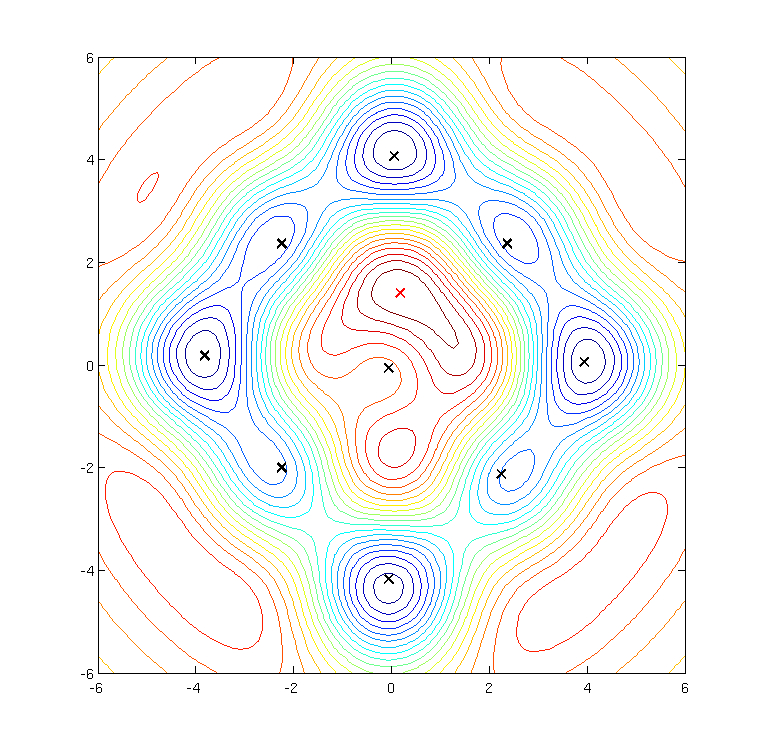
\includegraphics[width=6cm]{figures/herd_movie/v2herd10}}
       		\only<11>{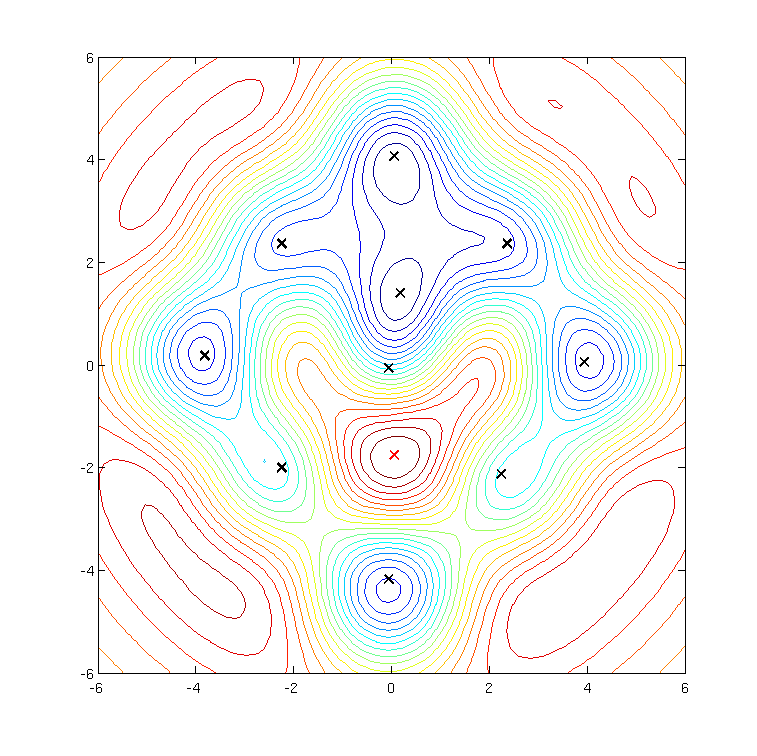
\includegraphics[width=6cm]{figures/herd_movie/v2herd11}}
       		\only<12>{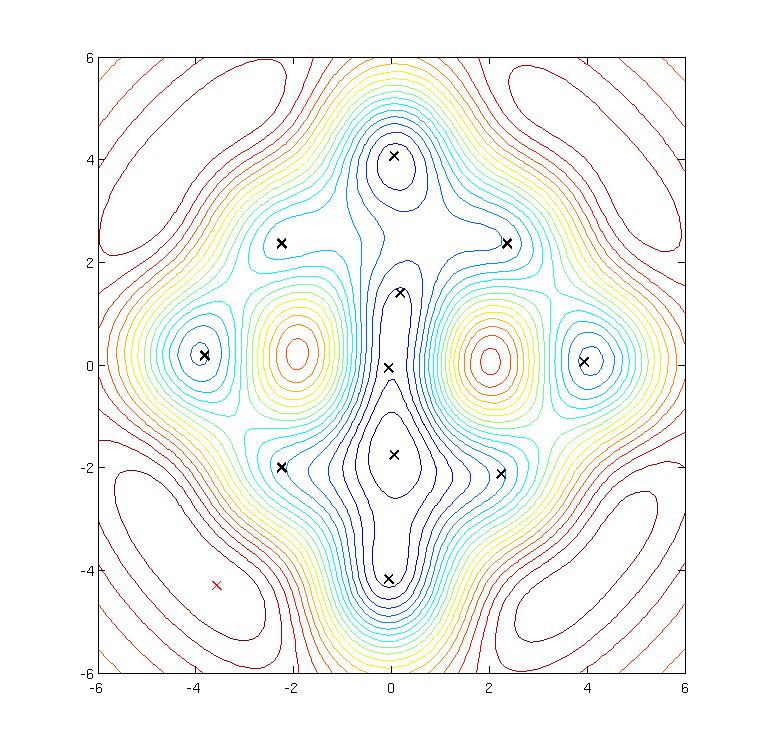
\includegraphics[width=6cm]{figures/herd_movie/v2herd12}}
       		\only<13>{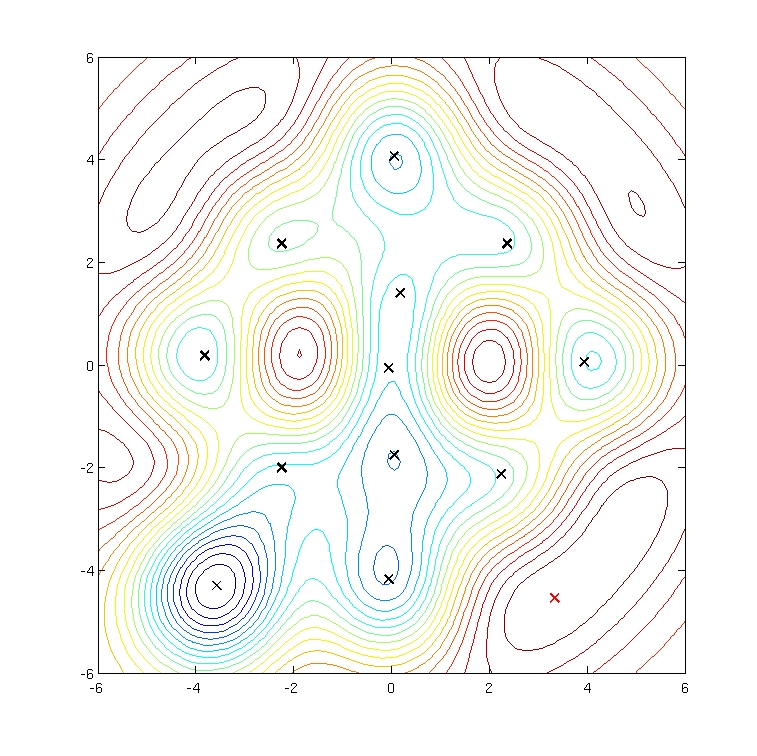
\includegraphics[width=6cm]{figures/herd_movie/v2herd13}}
       		\only<14>{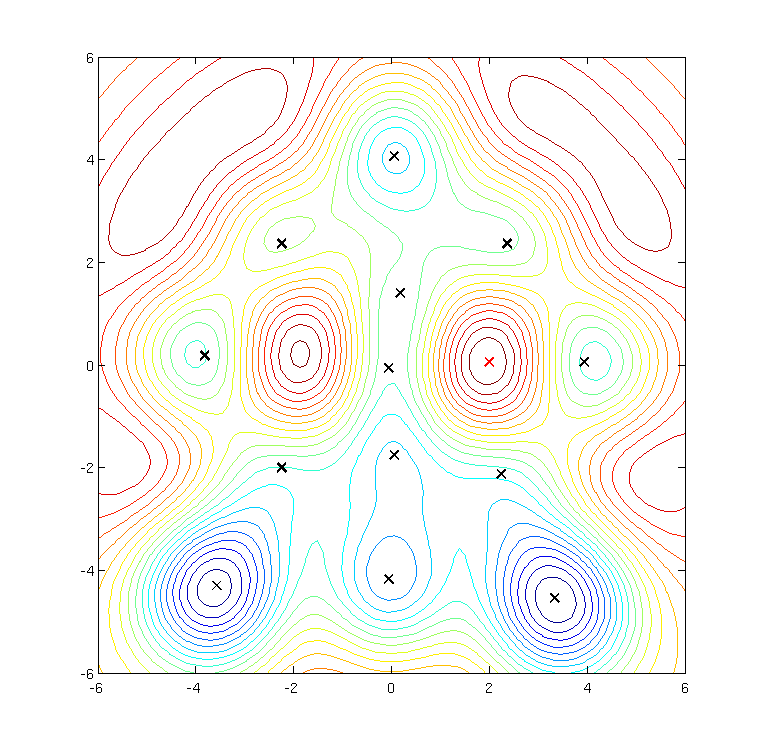
\includegraphics[width=6cm]{figures/herd_movie/v2herd14}}
       		\only<15>{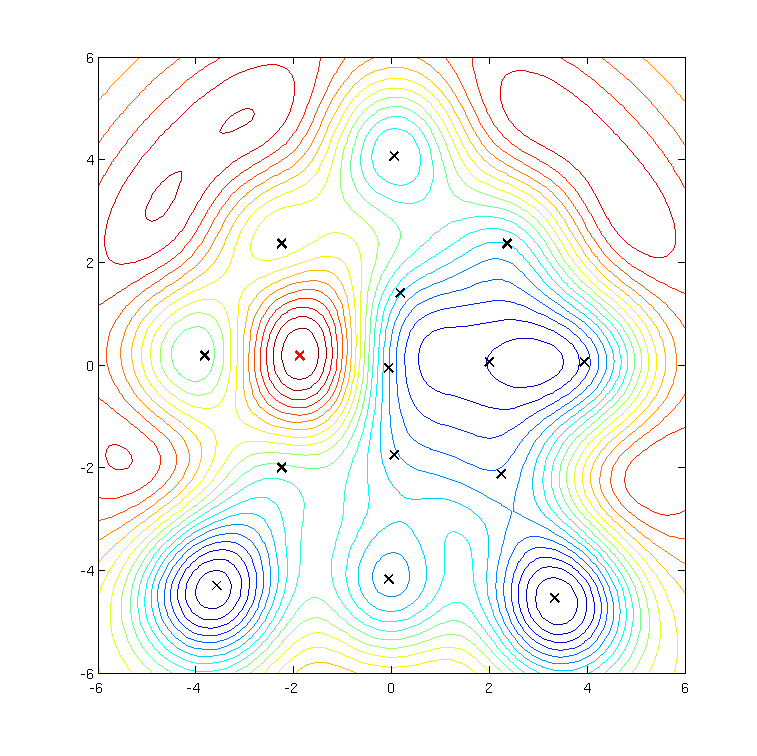
\includegraphics[width=6cm]{figures/herd_movie/v2herd15}}
       		\only<16>{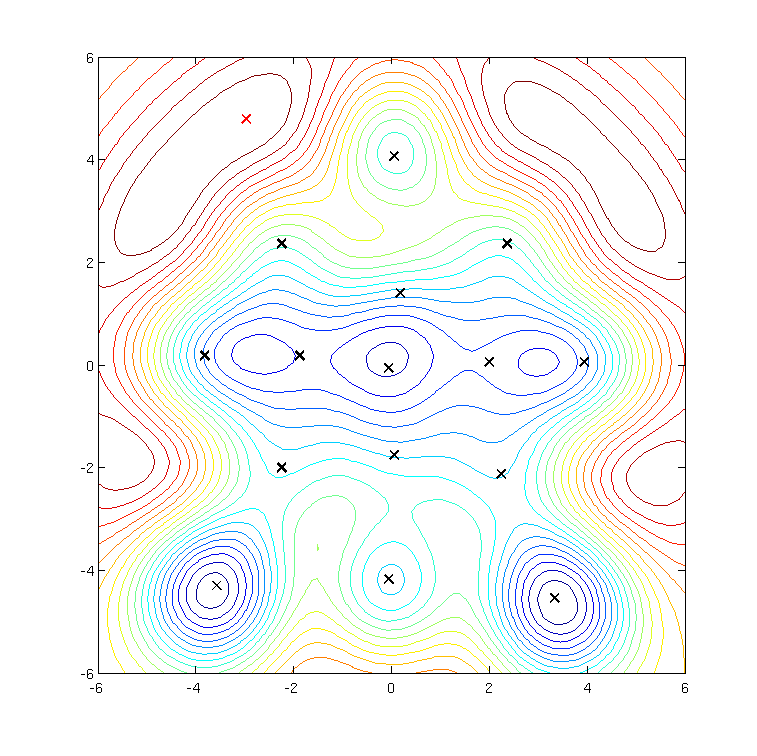
\includegraphics[width=6cm]{figures/herd_movie/v2herd16}}
       		\only<17>{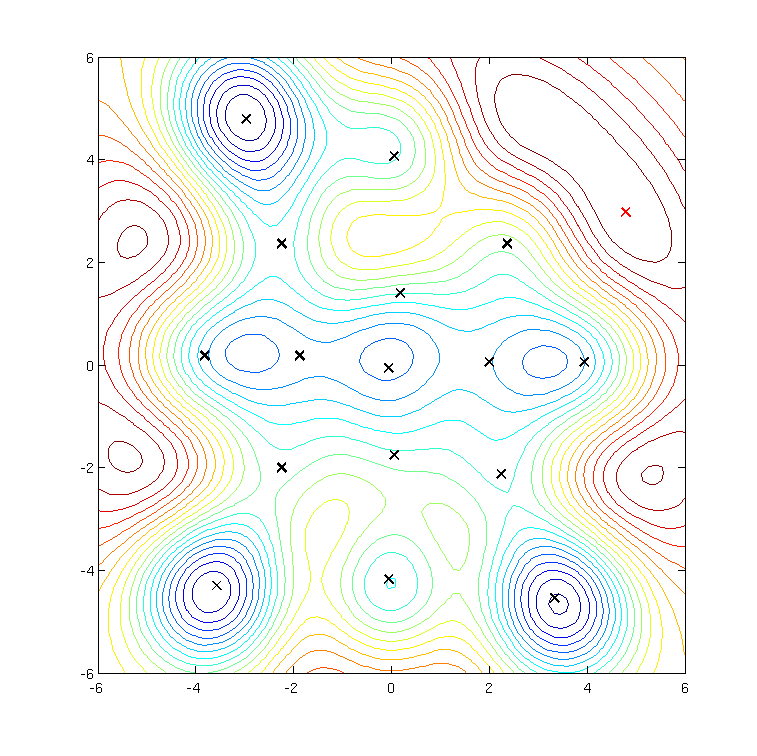
\includegraphics[width=6cm]{figures/herd_movie/v2herd17}}
       		\only<18>{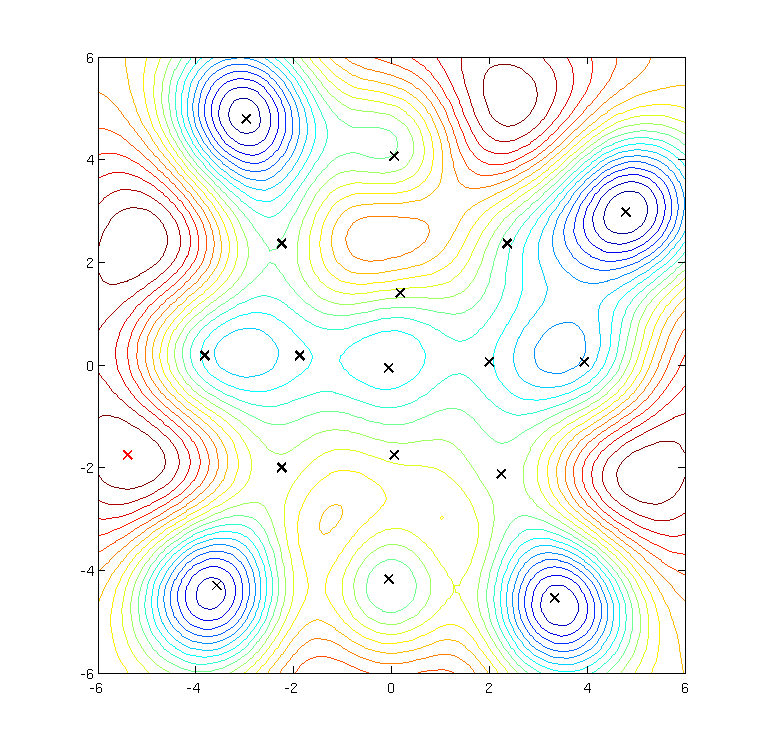
\includegraphics[width=6cm]{figures/herd_movie/v2herd18}}
       		\only<19>{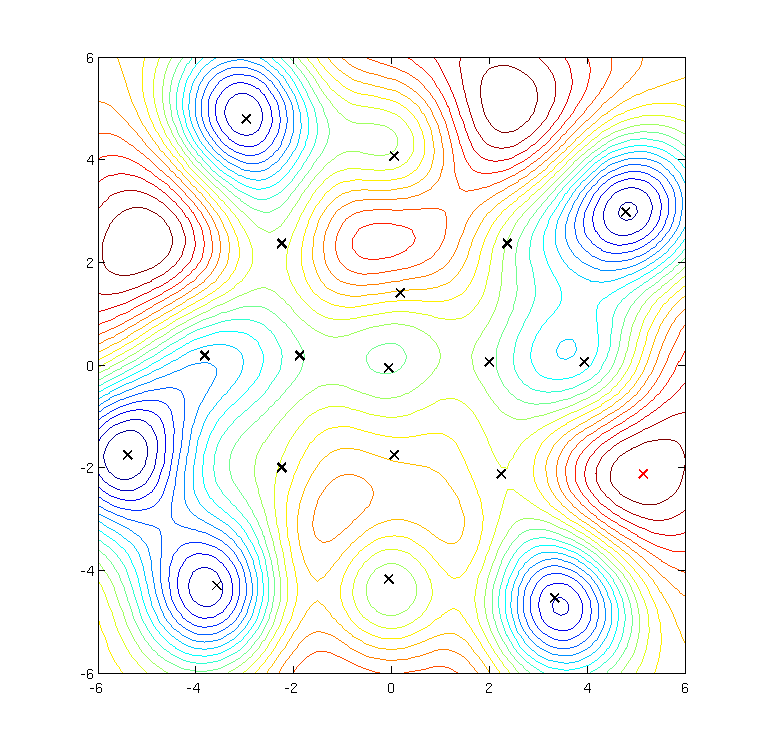
\includegraphics[width=6cm]{figures/herd_movie/v2herd19}}
       		\only<20>{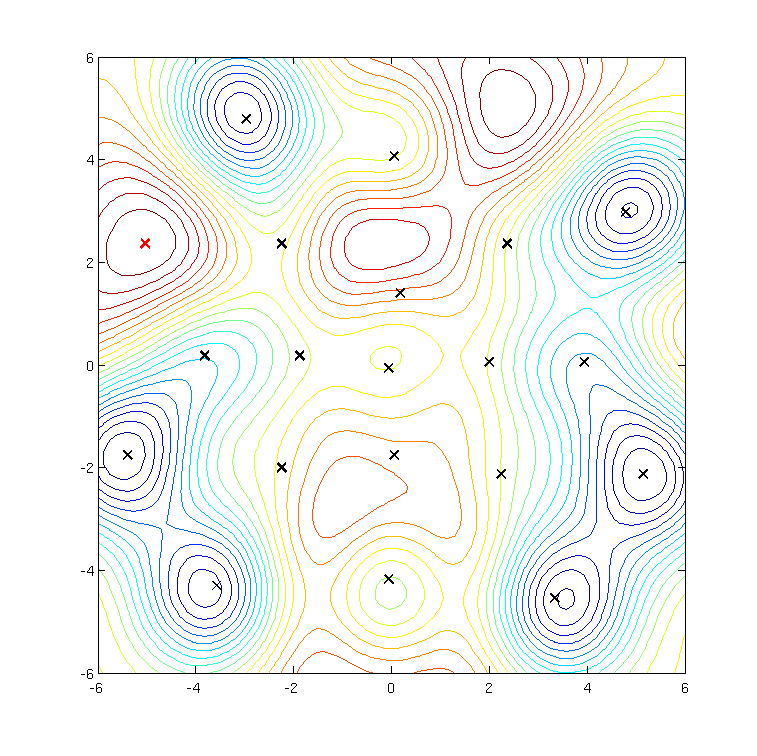
\includegraphics[width=6cm]{figures/herd_movie/v2herd20}}
		}
	}
	%
%	\takeaway%
%{
%	Takeaway
%}
\end{frame}






\begin{frame}[plain, t]
	\frametitleJL{Kernel Herding Summary}
	%
	\titlebodyskip
	%
	\bodyheaderskip
	%
	\slidebody
	{
			\begin{itemize}
				\item A sequential sampling method which minimizes a worst-case divergence, given that $f(x)$ belongs to a given RKHS.
				\item Like Monte Carlo, weights all samples $f(x_s)$ equally when estimating $Z$:  $$\hat{Z} =  \sum_{i=1}^N \frac{1}{N} f(x_i)$$
				\pause
				\item What if we allowed different weights?
				\pause
				\item {\color{mydarkblue} [Bach et. al. 2012]} looked at weighted herding strategies, showed improvement in convergence rates.
%				\item Enforced that weights are positive and sum to one.
%				\pause 
%				\item A natural thing to do, but is actually unnecessary.
				\pause
			\end{itemize}   		
	}
	%
	
	\vspace{0.5in}
	
	\takeaway%
	{
		Can we reason about the optimal weighting strategy?
	}
\end{frame}


\begin{frame}[plain, t]
	\frametitleJL{Bayesian Quadrature (a.k.a. Bayesian Monte Carlo)}
	%
	\titlebodyskip
	%
	\headerbar
	{
%		\columnheader{\standardtwocolumnwidth}
%		{
%			Simple Monte Carlo
%		}
		%
%		\spacer{\standardspace}
		%
%		\columnheader{\standardtwocolumnwidth}
%		{
%			Simple Monte Carlo
%		}
	}
	%
	\bodyheaderskip
	%
	\slidebody
	{
%		\columnbody{\standardtwocolumnwidth}
%		{	
		{\color{mydarkblue}[O'Hagan 1987, Diaconis 1988, Rasmussen \& Ghahramani 2003]	}
			\begin{itemize}
			
			\pause
				\item Places a GP prior on $f$, defined by $k(\cdot, \cdot)$ and a mean function.
				\item Posterior over $f$ implies posterior over $Z$.
				
%		}
		%
%		\spacer{\standardspace}
		%
%		\columnbody{\standardtwocolumnwidth}
%		{
%			\vskip10pt
%			\centering
       		\only<2>{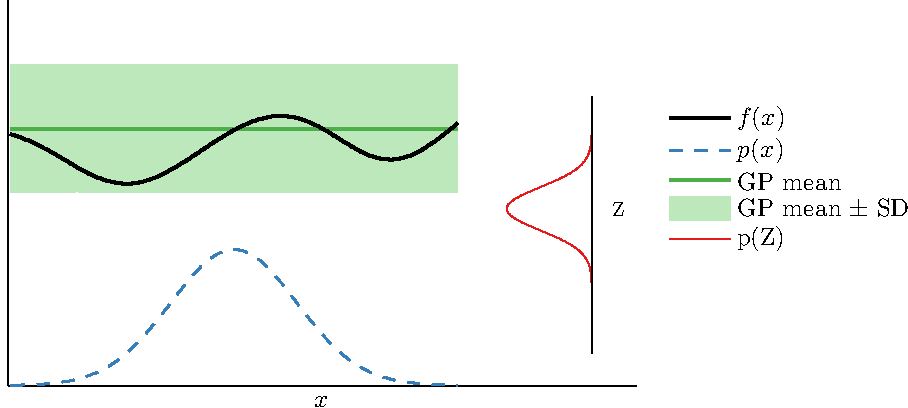
\includegraphics[width=10cm]{figures/bq_buildup/buildup_nosamps0}}
       		\only<3>{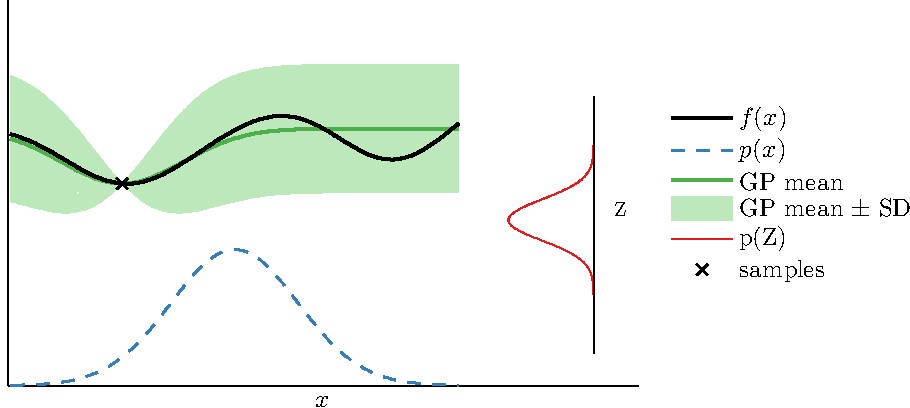
\includegraphics[width=10cm]{figures/bq_buildup/buildup_samps1}}
       		\only<4>{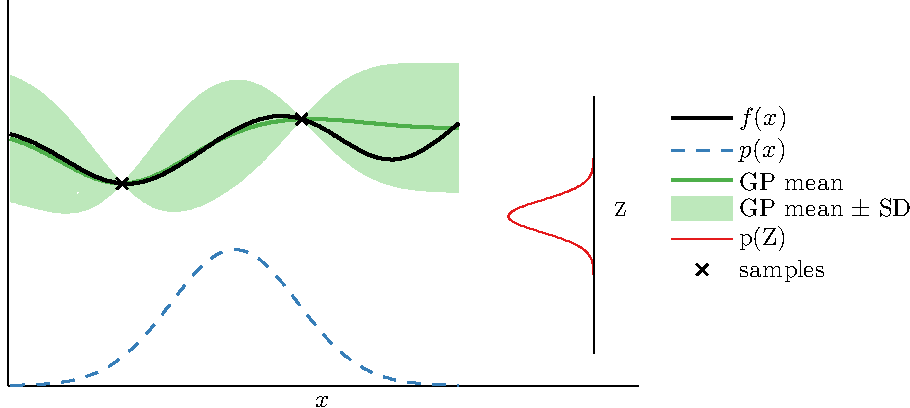
\includegraphics[width=10cm]{figures/bq_buildup/buildup_samps2}}
       		\only<5>{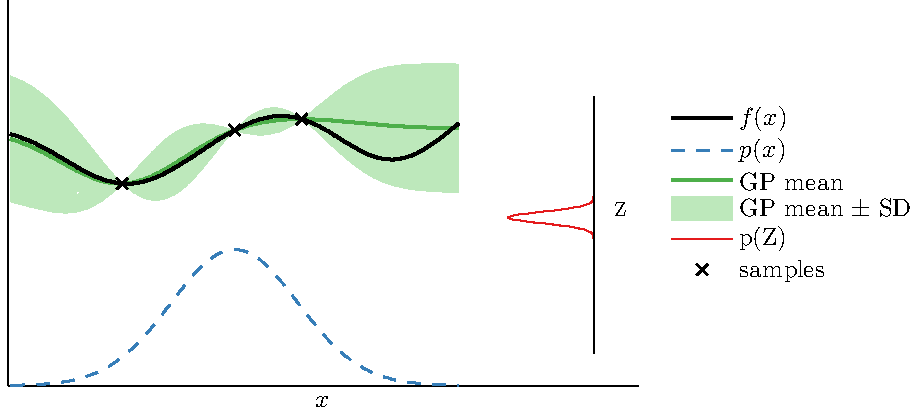
\includegraphics[width=10cm]{figures/bq_buildup/buildup_samps3}}
       		\only<6>{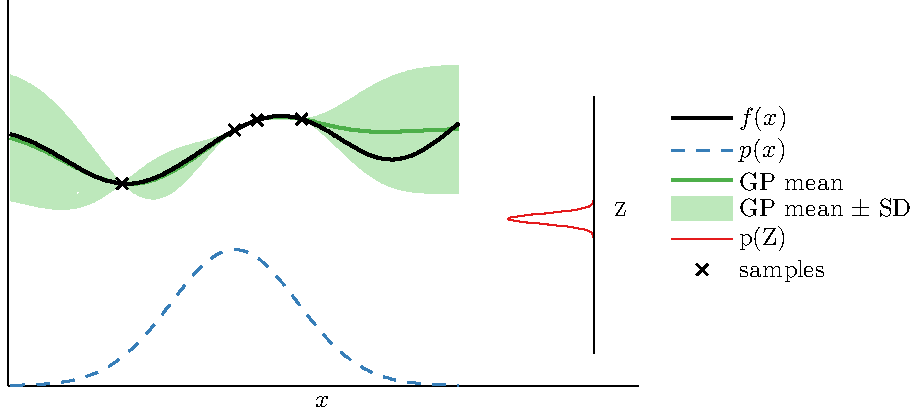
\includegraphics[width=10cm]{figures/bq_buildup/buildup_samps4}}       		      
       		\only<7-8>{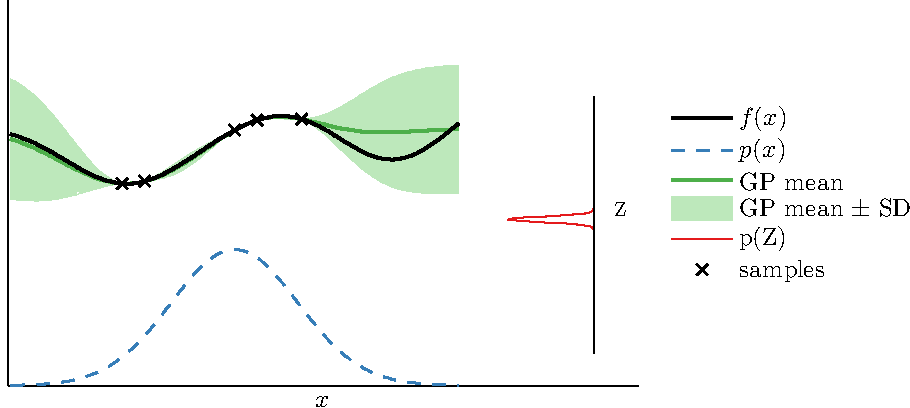
\includegraphics[width=10cm]{figures/bq_buildup/buildup_samps5}}
       		\only<8>{
       		\item Can choose samples however we want.}
			\end{itemize}   		
%		}
	}
	%
%	\takeaway%
%{
%	Takeaway
%}
\end{frame}



\begin{frame}[plain, t]
	\frametitleJL{Bayesian Quadrature Estimator}
	%
	\titlebodyskip
	%
%	\headerbar
%	{
%		\columnheader{\standardtwocolumnwidth}
%		{
%			Expectation of $Z$
%		}
		%
%		\spacer{\standardspace}
		%
%	}
	%
%	\bodyheaderskip
	%
%	\slidebody
%	{
%		\columnbody{\standardtwocolumnwidth}
%		{		

Posterior over $Z$ has mean linear in $f(x_s)$:
\begin{align*}
\expectargs{\gp}{Z|f(x_s)} %& = \expectargs{\gp}{\int f(\vx)p(\vx)d\vx} \\
% & = \int\!\!\! \int\!\! f(\vx) p(\vx) d\vx p(f(\vx)|\vf(\vx_s)) df\\
  & = \sum_{i=1}^N w_{\small{BQ}}^{(i)} \vf(\vx_i)
  \end{align*}
  where
  \begin{align*} 
% & = \int\!\!\! \int\!\! f(\vx) p(\vx) d\vx p(f(\vx)|\vf(\vx_s)) df\\
% & = \int\!\!\! \mf(\vx) p(\vx) d\vx df \\
% & = \left[ \int\!\! k(\vx, \vX) p(\vx) d\vx \right] K^{-1} \vf(\vX) \\
 w_{\small{BQ}} & = \vz^T K\inv \qquad \textrm{and} \qquad z_n = \int\!\! k(\vx, \vx_n) p(\vx) d\vx
\end{align*} 
\pause
%Weights are nonuniform, not necessarily positive.
\centering
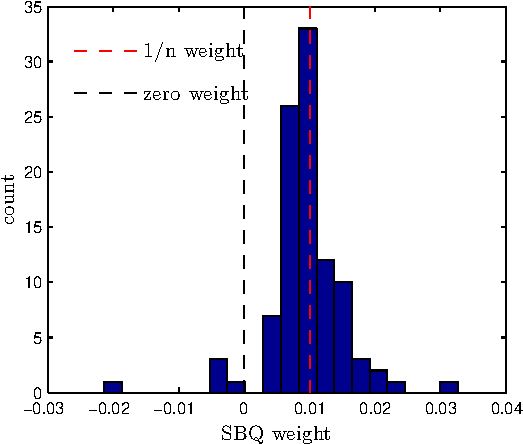
\includegraphics[width=0.45\columnwidth]{figures/weights_v1_n100}

%\end{align}
%		}
%	}
	%
%	\takeaway%
%{
	%\pause What is relation to herding?
%}
\end{frame}


\begin{frame}[plain, t]
	\frametitleJL{How to select samples?}
	%
	\titlebodyskip
	%
%	\headerbar
%	{
%		\columnheader{\standardtwocolumnwidth}
%		{
%			Expectation of $Z$
%		}
		%
%		\spacer{\standardspace}
		%
%	}
	%
%	\bodyheaderskip
	%
%	\slidebody
%	{
%		\columnbody{\standardtwocolumnwidth}
%		{		
\pause
\begin{itemize}
\item Natural to minimize the posterior variance of $Z$:
%$$\varianceargs{}{Z|f(x_s)} = \expectargs{\vx, \vx' \sim p}{k(\vx, \vx')} - \vz^T K\inv \vz$$
\begin{align*}
\varianceargs{}{Z|f(x_s)} & = \int \! \! \int \! k(\vx, \vx') p(x) p(x') dx dx' - \vz^T K\inv \vz \\
& \textrm{where} \qquad z_n = \int\!\! k(\vx, \vx_n) p(\vx) d\vx
\end{align*}
\pause
\item Favours samples in regions where $p(x)$ is high, but where covariance with other sample locations is low.  Similar flavour to herding objective.
\pause
\item Does not depend on function values
\pause
\item Can choose samples sequentially: Sequential Bayesian Quadrature.
\end{itemize}

%		}
%	}
	
%	\takeaway%
%{
%	\pause What is precise relation to herding?
%}
\end{frame}


\definecolor{lightblue}{rgb}{0.9,0.9, 1} 
\setbeamercolor{block title}{bg=blue,fg=white}%bg=background, fg= foreground
\setbeamercolor{block body}{bg=lightblue,fg=black}%bg=background, fg= foreground

\begin{frame}[plain, t]
	\frametitleJL{Relating Objectives}
	%
	\titlebodyskip
	%
%	\headerbar
%	{
%		\columnheader{\standardtwocolumnwidth}
%		{
%			Herding [cite]
%		}
		%
%		\spacer{\standardspace}
		%
%		\columnheader{\standardtwocolumnwidth}
%		{
%			Kernel Herding [cite]
%		}
%	}
	%
%	\bodyheaderskip
	%
 \slidebody
	{
	%	\columnbody{11cm}
	%	{		

		KH and BQ have completely different motivations:
		\begin{itemize}
			\item KH minimizes a worst-case bound
			\item BQ minimizes a posterior variance
		\end{itemize}
		Is there any correspondence?
	\pause
	\begin{block}{First Main Result}
	\begin{align*}
		\varianceargs{}{Z \vert f(x_s)} = \mmd^2(p,q_{\bq{}})
	\end{align*}		

		%How to compare the two?
		%\pause
		
		Where  $$q_{\bq{}}(x) = \sum_{n=1}^{N}w^{(n)}_{\bq{}}\delta_{x_n}(x)$$ 
	\end{block}		
		%under the RKHS defined by the covariance function of GP prior.
%		\pause
%		Then, $\mmd(p, q_{\bq{}})$ is identical to the GP posterior variance:
%The expected variance in the Bayesian quadrature estimate $\varianceargs{}{Z_{f,p}}$ is exactly the squared maximum mean discrepancy between the target distribution $p$ and BQ weighted ``distribution'' $q_{\bq{}}(x) = \sum_{n=1}^{N}w^{(n)}_{\bq{}}\delta_{x_n}(x)$:

	%	}
	}
	\pause
	
	\vspace{0.7in}
%	Frequentist and Bayesian criteria are identical!	

	\takeaway
{
BQ is minimizing KH objective
}
\end{frame}



\begin{frame}[plain, t]
	\frametitleJL{Performance}
	%
	\titlebodyskip
	%
%	\headerbar
%	{
%		\columnheader{\standardtwocolumnwidth}
%		{
%			Herding [cite]
%		}
		%
%		\spacer{\standardspace}
		%
%		\columnheader{\standardtwocolumnwidth}
%		{
%			Kernel Herding [cite]
%		}
%	}
	%
%	\bodyheaderskip
	%
	\slidebody
	{
	%	\columnbody{11cm}
%		{
\begin{itemize}
		\item KH and BQ are minimizing the same objective, but BQ has freedom to choose weights.% So, it can presumably do better.
		\pause
		\item How does this affect performance?
	    \pause 

	\begin{block}{Second Main Result}
	BQ estimator is the optimal weighting strategy:
\begin{align*}
\varianceargs{}{Z\vert f(x_s)} = \inf_{\bm{w}\in\mathbb{R}^N} \sup_{\substack{f\in\He\\\Hnorm{f}{\He}=1}} \left| \int f(x) p(x) dx - \sum_{n=1}^{N}w_n 	f(x_n)\right|^2
\end{align*}
\end{block}
\pause

$\varianceargs{}{Z\vert f(x_s)}$ has two interpretations:
\item Bayesian: posterior variance of Z under a GP prior.
\item Frequentist: tight bound on estimation error of Z.
\end{itemize}
%		}
	}
	%
%	\takeaway%
%{

	
%}
\end{frame}





\begin{frame}[plain, t]
	\frametitleJL{Rates of Convergence}
	%
	\titlebodyskip
	%
	
	What is rate of convergence of BQ?
	\headerbar
	{
		\columnheader{\standardtwocolumnwidth}
		{
			Expected Variance / MMD
		}
		%
		\spacer{\standardspace}
		%
		\columnheader{\standardtwocolumnwidth}
		{
			\only<4>{Empirical Rates in RKHS}
			\only<5>{Empirical Rates out of RKHS}
			\only<6>{Bound on Bayesian Error}		
		}
	}
	%
	\bodyheaderskip
	%
	\slidebody
	{
		\columnbody{\standardtwocolumnwidth}
		{		
			\vskip10pt
			\only<1>{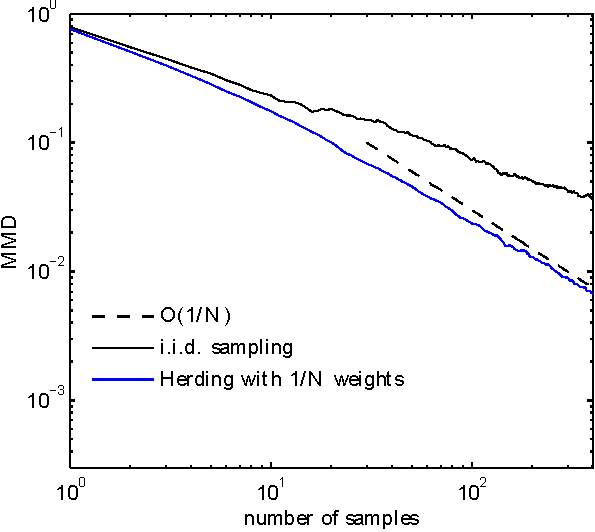
\includegraphics[width=\columnwidth]{figures/expected_variance_v7_400_no2}}	
			\only<2>{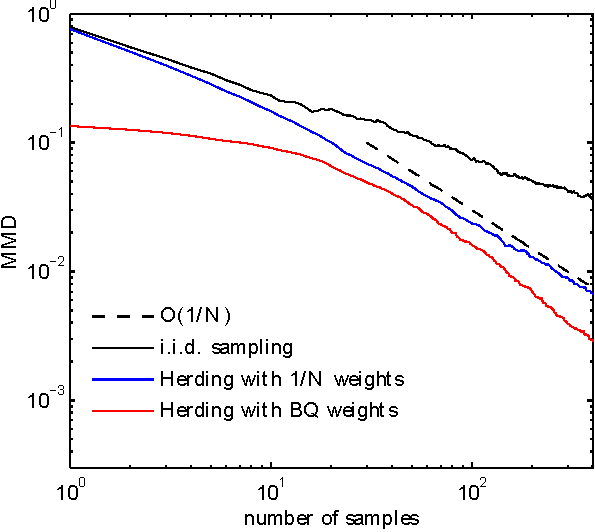
\includegraphics[width=\columnwidth]{figures/expected_variance_v7_400_no1}}		
			\only<3-6>{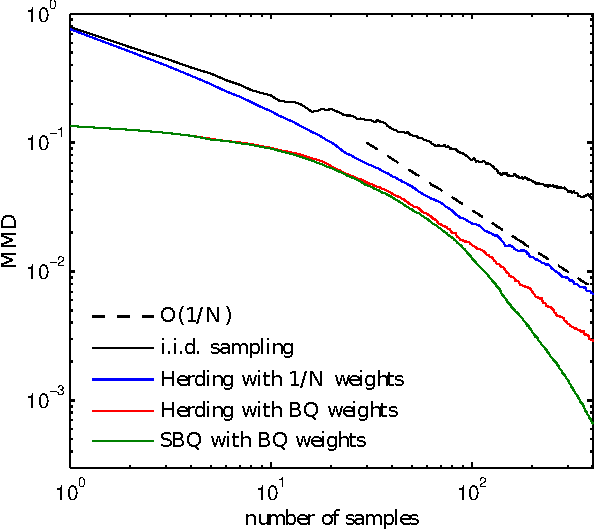
\includegraphics[width=\columnwidth]{figures/expected_variance_v7_400_no0}}					
		}
		%
		\spacer{\standardspace}
		%
		\columnbody{\standardtwocolumnwidth}
		{
			\vskip10pt
			\only<4>{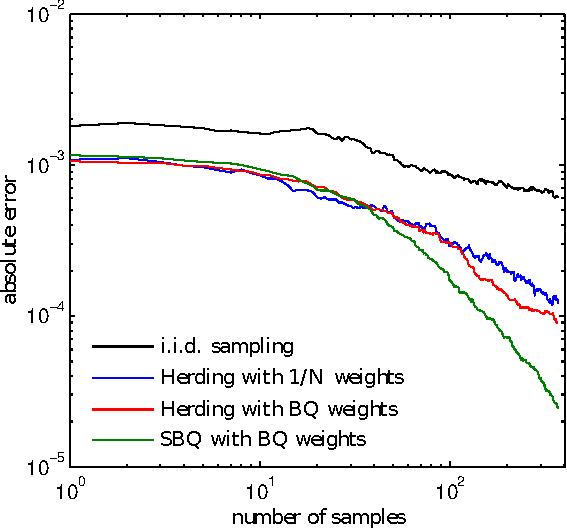
\includegraphics[width=\columnwidth]{figures/error_curve_outmodel_400_v3}}
			\only<5>{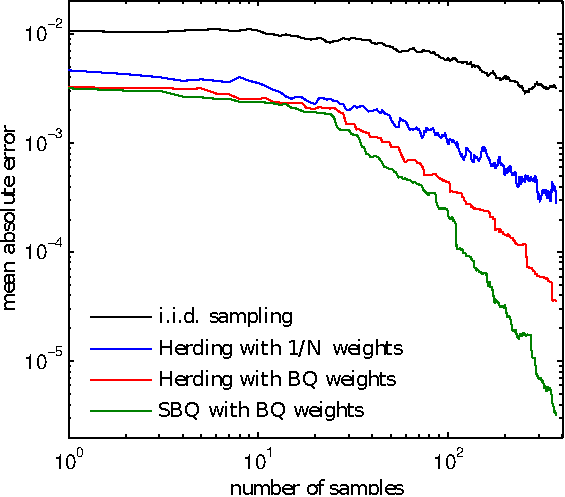
\includegraphics[width=\columnwidth]{figures/error_curve_rkhs_400_v4}}
			\only<6>{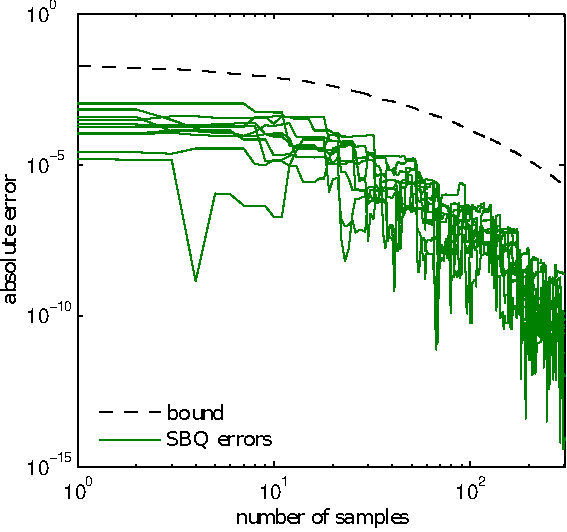
\includegraphics[width=\columnwidth]{figures/bound_curve_rkhs}}			
		}
	}
	%
%	\takeaway%
%{
%	Takeaway
%}
\end{frame}


\begin{frame}[plain, t]
	\frametitleJL{Summary}
	%
	\titlebodyskip
	%
	\headerbar
	{
		%\columnheader{\standardtwocolumnwidth}
		%{
	%		About Sampling
%		}
		%
%		\spacer{\standardspace}
		%
%		\columnheader{\standardtwocolumnwidth}
%		{
%			In General
%		}
	}
	%
	\bodyheaderskip
	%
	\slidebody
	{
%		\columnbody{\standardtwocolumnwidth}
%		{
			\begin{itemize}
				\item Posterior variance of Z under GP prior is equivalent to Maximum Mean Discrepancy.
				\pause
				\item RKHS assumption gives a tight, closed-form upper bound on Bayesian error.
				\pause
				\item BQ has very fast, but unknown convergence rate.
				\pause
				\item The optimal weighted herding strategy is Bayesian quadrature.
				\pause
				\item Joint work with Ferenc Huzsar
%				\begin{itemize}
%					\item BQ has higher complexity than KH ( $\mathcal{O}(N^3)$ versus $\mathcal{O}(N^2)$) but requires fewer samples.
%					\end{itemize}
%				\pause
		%	\end{itemize}	
%		}
		%
%		\spacer{\standardspace}
		%
%		\columnbody{\standardtwocolumnwidth}
%		{
		%	\begin{itemize}
%				\item Bayesian method has a minimax interpretation.
%				\pause
			\end{itemize}					
%		}
	}
	%
%	\takeaway%
%{
%	Thanks!
%}
\end{frame}


\end{document}

